\chapter{Introducing Deep Neural Networks into the COACH Framework}
In this chapter, we propose to extend the use of human corrective feedback during task execution to learn policies with state spaces of low and high dimensionality in $\text{continuous-action}$ problems using deep neural networks.

We combine Deep Learning (DL) with the corrective advice based learning framework called COrrective Advice Communicated by Humans (COACH) \cite{Celemin2018AnInteractive}, thus creating the Deep COACH (D-COACH) framework. In this approach, no reward functions are needed and the amount of learning episodes is significantly reduced in comparison to alternative Reinforcement Learning (RL) approaches.

\section{Overview}
In previous years, learning algorithms for solving sequential decision-making problems heavily relied on carefully handcrafted features based on human intuition and knowledge about them to obtain good performances. Also, when using linear combination of basis functions (LCBFs) as function approximator, which was one of the most commonly used function approximator, for each problem it was necessary to select a specific set of basis functions. Choosing a well performing set of basis functions is a process that may require expert knowledge or several tests, which may become very time consuming or unfeasible as the size of the $\text{state-action}$ space increases. This is also a consequence of the \emph{Curse of Dimensionality} \cite{bellman2003dynamic} which states that as the number of the dimensions of a space grows (state and/or action spaces in this case), exponentially more data and computation is needed to completely cover it. In LCBFs, this often means that their number of parameters $\theta$ grows exponentially as the number of dimensions increase. As a consequence, for most of the cases, learning algorithms needed handcrafted features in low-dimensional state spaces to adequately converge.

Given that COACH uses LCBFs as function approximator, it does not scale up well to problems with high-dimensional state spaces. However, the ideas proposed in COACH for shaping policies are independent of the function approximator that is used. With nowadays techniques, it has been shown that by approximating policies with Deep Neural Networks (DNNs) it is possible to solve problems with high-dimensional state spaces and with unprocessed raw information. So it seems as a natural step to extrapolate the ideas proposed in COACH to DNNs. 

\section{Methodology}
COACH is an algorithm designed to work with LCBFs that has different versions and variations. Consequently, in order to extrapolate its ideas to DNNs, it is necessary to see which of those can be used and why.

Given that in this thesis we are introducing the first approach that combines COACH with DNNs, we decided to design an algorithm based on the basic structure of COACH, shown in Algorithm \ref{algorithm:COACH} (Chapter \ref{sss:COACH}). We believe that there is still space to incorporate more ideas into D-COACH using the work presented in this thesis as a first step for future research.

The basic structure of COACH proposes two main ideas:

\begin{enumerate}
    \item \textbf{Using corrective feedback to shape policies:} COACH was built from this idea, so using it is a requirement. D-COACH uses corrective feedback \emph{almost} exactly as COACH. In COACH, it is proposed that each dimension of the action space should be trained independently, which has the advantage of creating a working framework that does not need any prior information about the problem in order to give corrections. We call this type of policy updating \emph{decoupled} training, so a correction in an specific action dimension does not modify the magnitude of the actions in other axes for the same corresponding state. However, in this work we consider that for some problems it may be advantageous to exploit prior user knowledge about relations between the different dimensions of the actions. In this way, a correction in one of the action axes may be used to update more than one dimension. We call this case \emph{coupled} training.
    
    \item \textbf{Using past corrections to modify the effects of newer ones:} In COACH, this idea is reflected in the Human Model; in D-COACH, a replay buffer (or experience replay, see Chapter \ref{sss:ER}) is incorporated into the algorithm, which is a technique that has been strongly validated with several DRL approaches \cite{atari, haarnoja2018soft, Lillicrap2015}. Even though both the Human Model and the replay buffer use information given by past corrections to modify the effects of newer ones, they do not do it in the same way. The Human Model modifies the learning rate of the policy adaptively; the replay buffer updates the policy constantly by replaying past corrections. Including a Human Model into $\text{D-COACH}$ could help with the dilemma of setting either a too large or too small learning rate for updating the weights of a policy. In this case, we did not include a Human Model because this would have meant to add a second DNN model in charge of learning it. As a consequence, the overhead of D-COACH would have increased and we prioritized a framework with fewer computational cost.
\end{enumerate}


\subsection{Low-Dimensional vs High-dimensional States}
When using DNNs, problems are often separated depending on the nature of their network inputs. When these inputs are processed data (such as handcrafted features in RL) a common approach is to use FNNs; When they are unprocessed raw information, CNNs are the most common option. In the RL context, given that the input of the networks is the state/observation of the environment, we use the term \emph{low-dimensional states} to refer to the input of the former, and \emph{high-dimensional states} to refer to the input of the later. Thus, FNNs are used in problems with low-dimensional state spaces and CNNs in problems with high-dimensional state spaces. Nevertheless, it is important to notice that handcrafted features are not necessarily low-dimensional and that FNNs may be also used in those cases. This is a commonly made association because the input of classic RL approaches were handcrafted features whose size was limited by the curse of dimensionality (and the computational power available at that time), and, as a consequence, they were low-dimensional.

Training CNN policies is a more challenging problem than training FNN policies. Both the state representation from raw data (this work focuses on applications with raw images as observation) and the policy must be learned from information interactively given by a human. DNNs have shown to need large sets of data and experience to adequately converge in complex problems, such as those with $\text{high-dimensional}$ inputs. The requirement of massive amounts of trials can be problematic because human users cannot keep on assisting the training for a long time due to stress, fatigue, or other factors that may lead to a lack of concentration.

To address this limitation, we employ \emph{state representation strategies} in problems with high-dimensional states/observations. The convolutional layers of a CNN can be interpreted as operations that extract the most relevant features out of a high-dimensional input. Thus, the output of these layers (which is commonly linked to a FNN in regression problems) can be seen as a representation of the state in a new space where the problem is easier to solve. This is what we call the state representation. So, in this context, state representation strategies refer to techniques employed for assisting the learning process of the state representation. In this work, the state representation of the policy is trained with additional criteria, adding an autoencoder to help with the training of the convolutional layers (or encoding layers) of the network.

\subsubsection{Offline State Representation Learning}
The D-COACH version introduced in this Chapter, OFFline state representation learning (D-COACH OFF), proposes to learn policies in a 3-step sequential process. In the first step, a session of demonstrations where observations of the environments are captured is recorded. Then, in a second step, the convolutional layers of the policy/autoencoder are trained with the recorded data, while tuning an  autoencoder  used  for state representation of reduced dimensionality, (Figure \ref{fig:ms}(a)). The state is embedded in the latent space of an autoencoder $\mathcal{L}$. Finally, in the third step, the convolutional layers of the trained encoder are frozen, then the subsequent non-convolutional layers (right hand side of Figure \ref{fig:ms}(b)) are trained interactively based on the corrections that the teacher advises to the agent. Figure \ref{fig:ms} depicts the second and third steps of this strategy. This kind of sequential strategy has been proven to work in decision-making problems \cite{Warnell2017,Finn2015,Ha2018}.

\begin{figure}[h]
\centering
\subfloat[][Autoencoder network for learning the state representation of the policy based on the demonstrations database.]{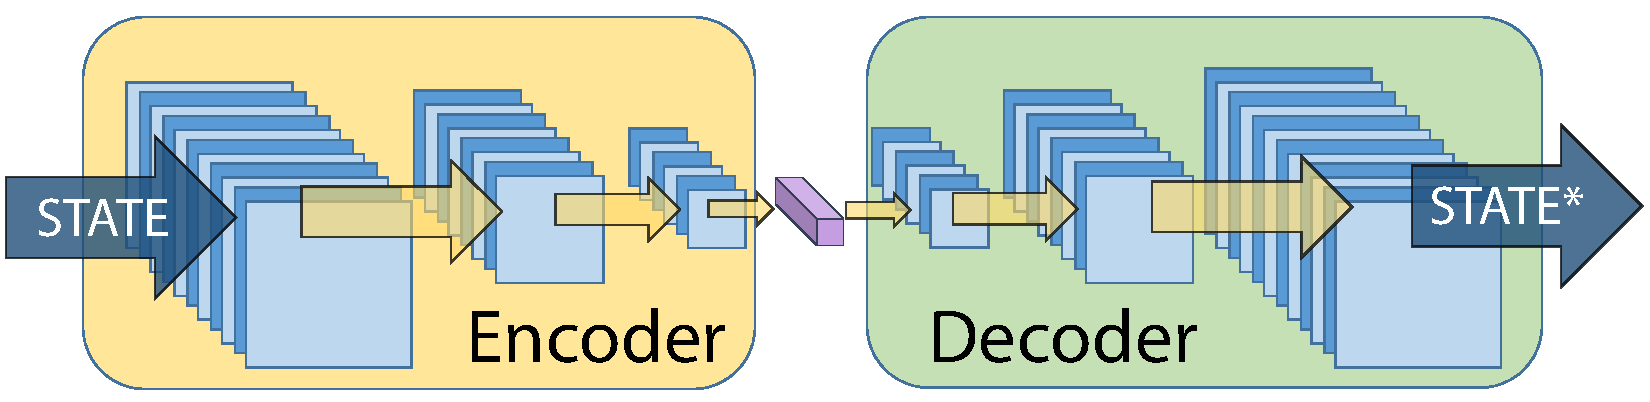
\includegraphics[width=0.45\linewidth]{imagenes/cap2/m1_p1.pdf}}
\hspace{0.1cm}
\subfloat[][Interactive training of the policy using the trained convolutional layers.]{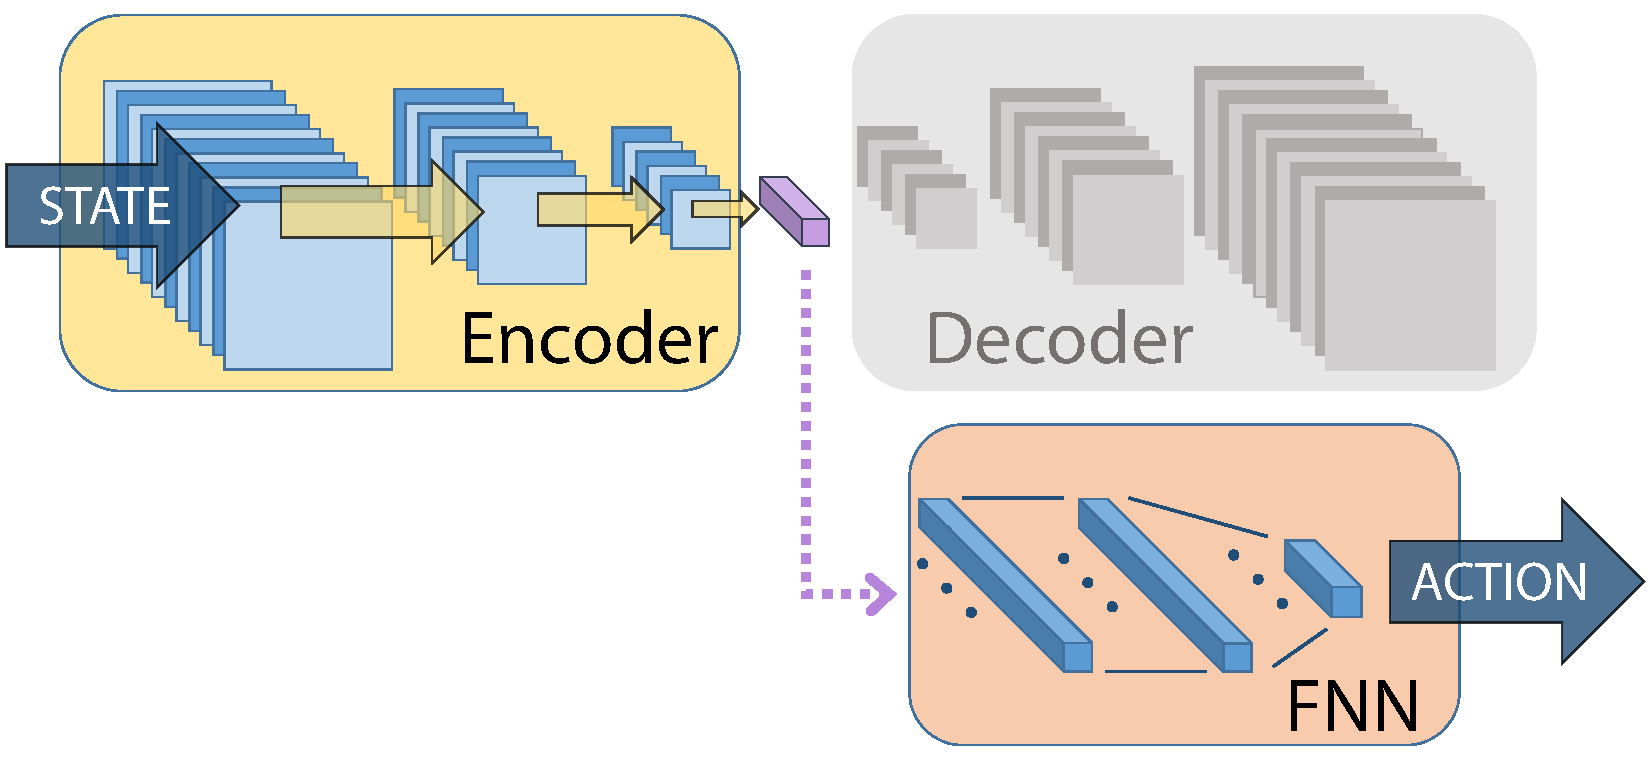
\includegraphics[width=0.45\linewidth]{imagenes/cap2/m1_p2.pdf}}
\caption{D-COACH OFF learning scheme.} 
\label{fig:ms} 
\end{figure}

In the case of low-dimensional state problems, the state is fed into a FNN (Policy), skipping the autoencoder related steps and training the policy with interactive feedback directly. Figure \ref{fig:network_diagram} summarizes the network architecture for both low-dimensional and high-dimensional state problems.

\begin{figure}[h]
    \centering
    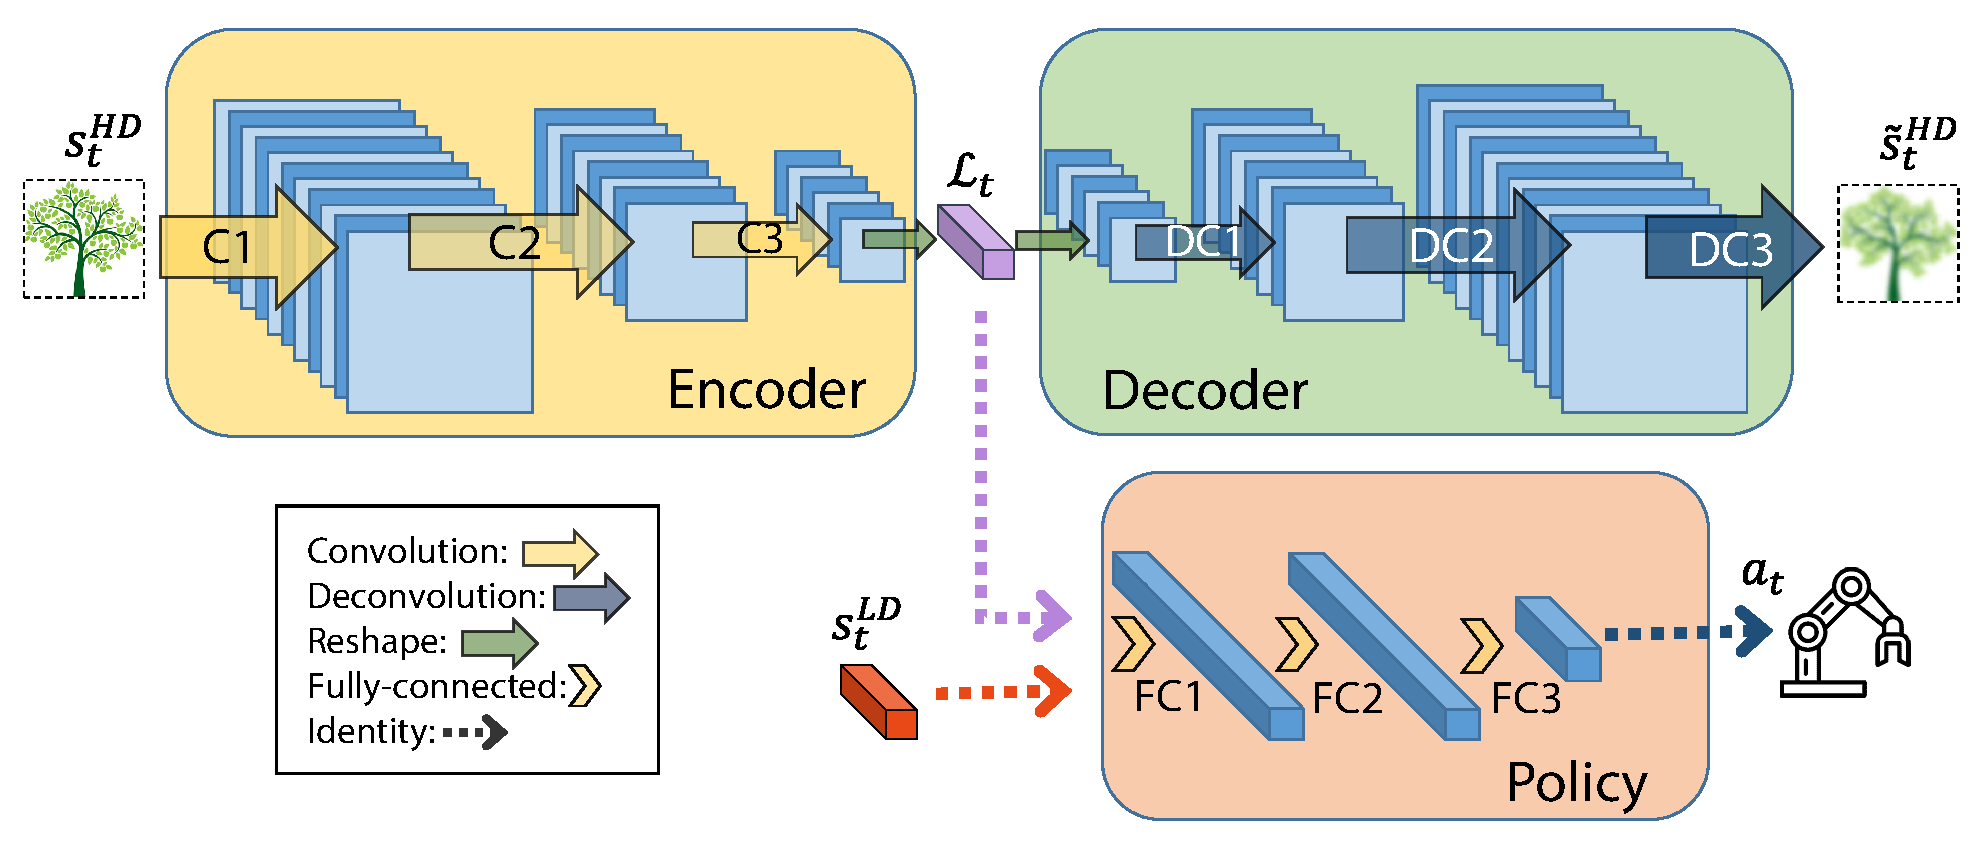
\includegraphics[width=\linewidth]{imagenes/cap2/ISER_diagram2.pdf}
    \caption[D-COACH OFF neural network architecture.]{D-COACH OFF neural network architecture. $s_{t}^{HD}$: high-dimensional state, input of the policy is the latent space of the autoencoder $\mathcal{L}_{t}$ (purple arrow). $s_{t}^{LD}$: low-dimensional state, input of the policy is the observed state (red arrow).}
    \label{fig:network_diagram}
\end{figure}

\subsection{The Algorithm}
In D-COACH, the policies are updated every time feedback is received and also by sampling from a memory buffer $\mathcal{B}$ with a fixed frequency every $b$ time steps. Every time the user advises a correction, the buffer $\mathcal{B}$ is fed with the current state and a label generated by adding the action taken with the error correction $y_{label}=a+\mathit{error}$.

The high-dimensional case can be seen as an extension of the low-dimensional case, where an offline state learning process must be added. Algorithm \ref{algorithm:DeepCOACH} presents the D-COACH OFF pseudocode.

\begin{algorithm}[h]
\caption{D-COACH OFF: Offline State Representation Learning}\label{algorithm:DeepCOACH}
\begin{algorithmic}[1]
\State \textbf{Require:} error magnitude $e$, buffer update interval $b$, buffer sampling size $N$, buffer min. size $k$, buffer max. size $K$, pre-trained encoder parameters (if convolutional) 
\State \textbf{Init:} $\mathcal{B} = []$  \emph{\# initialize memory buffer}
\For{t = 1,2,...}{}
\State \textbf{observe} state $s_{t}$
\State \textbf{execute} action $a_{t}=\pi(s_{t})$
\State \textbf{feedback} human corrective advice $h_{t}$
\If{$h_{t}$ is not \textbf{0}}
\State $\mathit{error}_{t} = h_{t}\cdot e$
\State $y_{label(t)} = a_{t} + \mathit{error}_{t}$ 
\State \textbf{update} $\pi(s)$ using SGD with pair ($s_{t}$, $y_{\mathit{label}(t)}$) 
\State \textbf{update} $\pi(s)$ using SGD with a mini-batch sampled from $\mathcal{B}$
\State \textbf{append} $(s_{t}, y_{\mathit{label}(t)})$ to $\mathcal{B}$
\If{length($\mathcal{B}$) $> K$ }
\State $\mathcal{B} = \mathcal{B}[2:K+1]$
\EndIf
\EndIf
\If{mod(t, b) is 0 and length($\mathcal{B}$) $\geq k$}
\State \textbf{update} $\pi(s)$ using SGD with a mini-batch sampled from $\mathcal{B}$
\EndIf
\EndFor
\end{algorithmic}
\end{algorithm}

\vspace{-0.1cm}
\section{Experiments and Results}
\vspace{-0.1cm}

Our proposed algorithm is validated experimentally in three different problems: 

\textbf{(i) Cart-Pole:} A simulated task with low-dimensional state space where the objective is to balance a pole attached to a cart (OpenAI gym implementation used \cite{brockman2016openai}) . The cart can only move in one axis with an acceleration value between $-1$ and $1$. The state has four dimensions, which consists of the position $x$ and velocity $\dot x$ of the cart, and the angle $\theta$ and angular velocity $\dot \theta$ of the pole. A representation of the Cart-Pole environment is presented in Figure \ref{fig:cartpole}.

\begin{figure}[h]
    \centering
    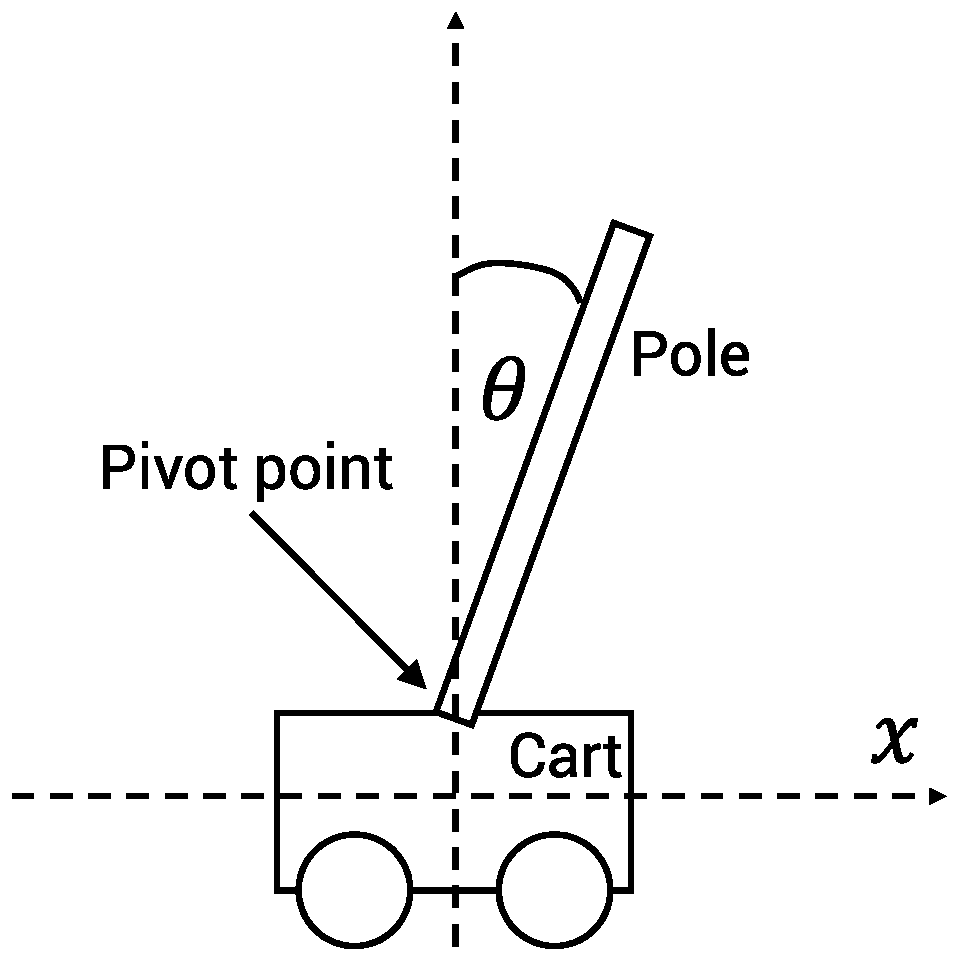
\includegraphics[scale=0.27]{imagenes/cap2/cartpole.pdf}
    \caption{Cart-Pole environment representation.}
    \label{fig:cartpole}
\end{figure}


\textbf{(ii) Car Racing:} A simulated problem (from OpenAI gym \cite{brockman2016openai}) in which the agent has to learn to drive from a top-down view of a racing car game (see Fig.~\ref{fig:Car_Racing}). The objective of the task is to drive a racetrack as fast as possible without leaving it. The default state that is given by the environment is a $96\times96\times3$ top-down view of the car which we downsampled to $64\times64\times1$. The continuous-action space consists of 3 dimensions: \textbf{(direction, acceleration, brake)}. The \emph{direction} range goes from $-1$ to $1$, the \emph{acceleration} from $0$ to $1$ and the \emph{brake} from $0$ to $1$.

\begin{figure}[h]
    \centering
    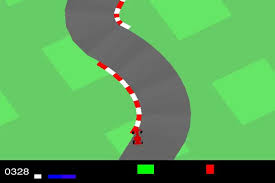
\includegraphics[scale=0.7]{imagenes/cap3/car_racing_env.jpg}
    \caption{Car Racing, environment view.}
    \label{fig:Car_Racing}
\end{figure}

\textbf{(iii) Duckie Racing:} This is also a driving task with high-dimensional input, but in this case with a robot, which has an onboard camera that gives a first-person view of the environment. The robot consist of a Duckiebot from the project Duckietown \cite{Paull2017}. A $120\times160\times3$ observation image is received from the environment which is downsampled to $64\times64\times1$. The duckiebot is a differential robot, so the default actions consisted of speed commands ranging from -1 to 1 for each of the two wheels. To make it more intuitive for a human teacher to give feedback, the environment had an inverse kinematics module for the actions to be linear and rotational speeds instead, also ranging from -1 to 1. A picture of the Duckiebot and its first-person view are shown in Figure \ref{fig:duckietown_off}.

\begin{figure}[h]
\centering
\subfloat[][Duckiebot.]{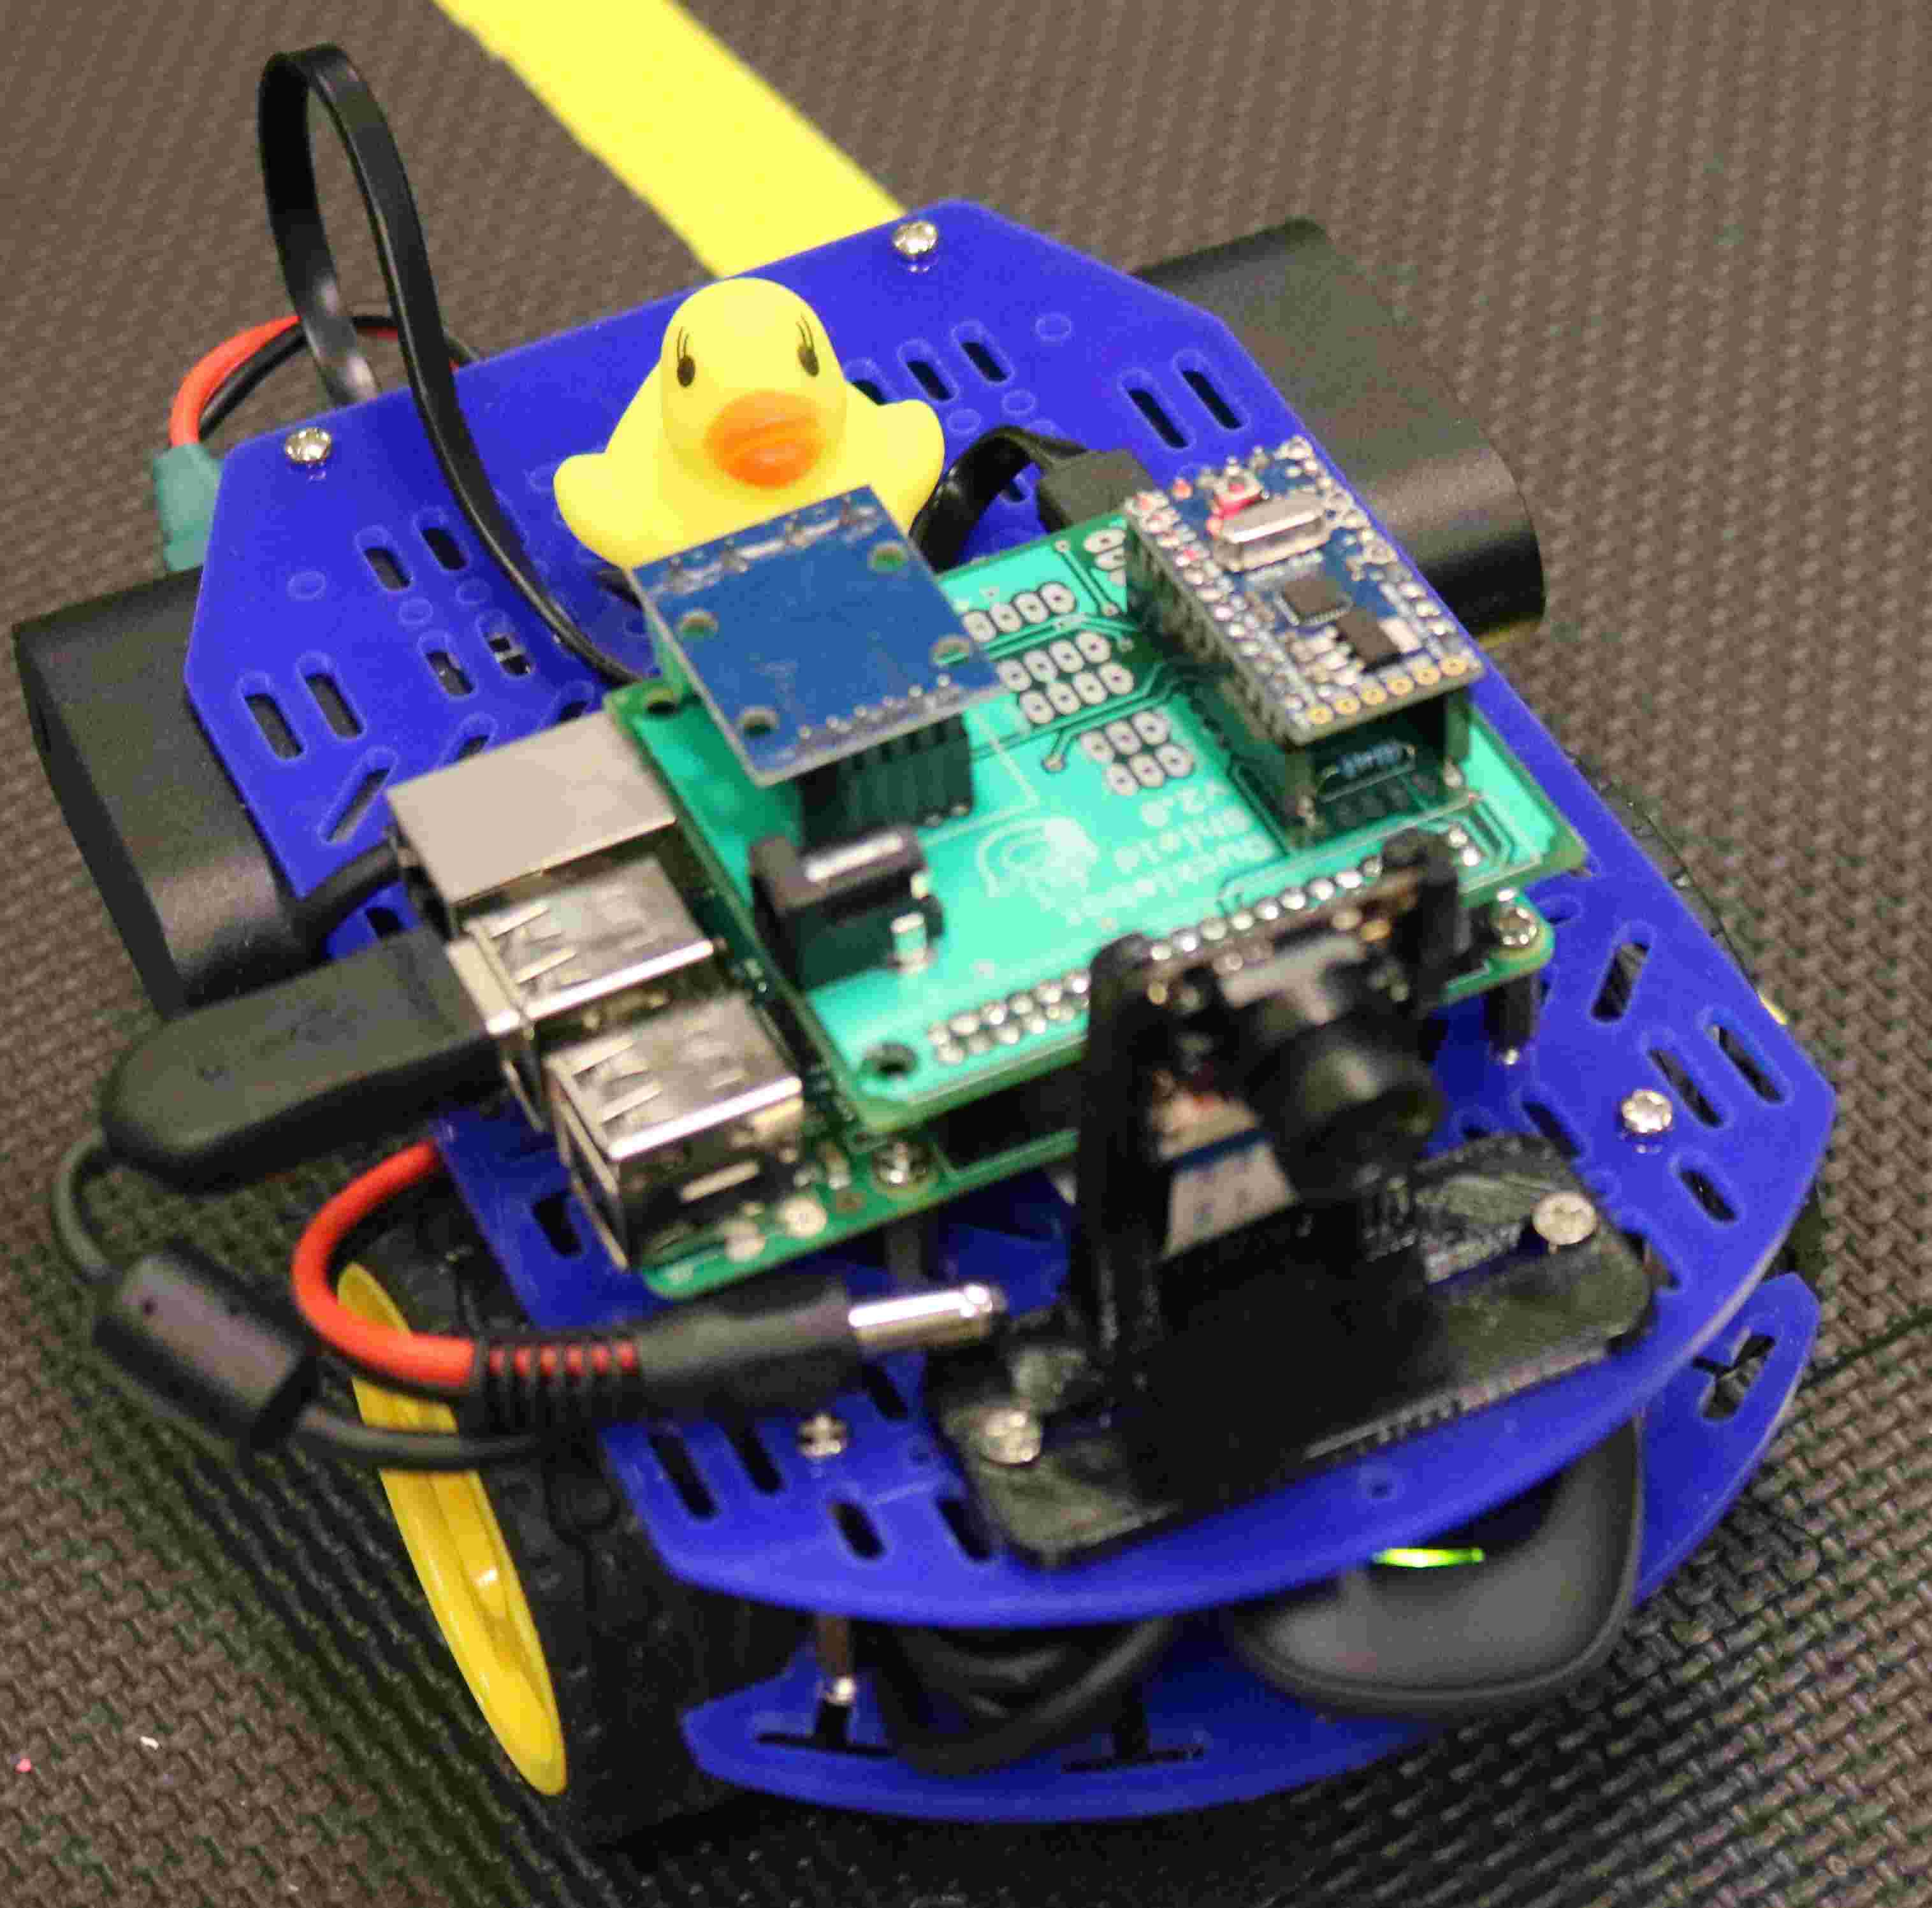
\includegraphics[width=0.305\linewidth]{imagenes/cap3/duckie_image.jpg}} 
\hspace{1.3cm}
\subfloat[][First-person view.]{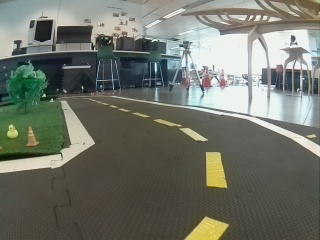
\includegraphics[width=0.4\linewidth]{imagenes/cap3/real_duckie_view.jpg}}
\caption{Duckietown D-COACH OFF.} 
\label{fig:duckietown_off} 
\end{figure}

The experiments were carried out using two types of teachers: (1) humans and (2) simulated teachers. Even though D-COACH is intended to work with humans, in order to evaluate the method along with subtle variants under more controlled conditions, a high performance policy standing-in as a teacher, which was actually trained with D-COACH and a real human teacher, was also used (similar approaches have been taken in \cite{Celemin2018AnInteractive, griffith2013policy}).

The experiments with simulated teachers are intended to compare the complete $\text{D-COACH}$ OFF presented in Algorithm \ref{algorithm:DeepCOACH}, along with a version of it without replay buffer (ignoring lines 2 and 11-16), and with a well known DRL algorithm Deep Deterministic Policy Gradient (DDPG) \cite{Lillicrap2015} (OpenAI \cite{baselines} implementation used), given that it is designed to work in continuous-action problems. The comparison is carried out by plotting the cumulative reward obtained at each episode by the agent as a function of time. In the case of $\text{D-COACH}$, the obtained reward is only used as a performance metric. Also, the results are presented as a function of time instead of episodes (except in the Duckie Racing experiment, where the maximum time that each episode can last is 30 seconds), because episodes can have variable duration depending on the policy. Hence, the episode scale would not properly show the time taken by the learning process, which is an important characteristic, since $\text{D-COACH}$ is meant to work with robots.

The simulated environments, Cart-Pole and Car Racing, were ran at $22.5$ and $20.5$ FPS, respectively. These experiments were carried out using human teachers and simulated teachers. Humans had approximately 5 minutes to practice teaching in each environment. The learning curves of agents trained by 10 human teachers were obtained and averaged; the learning curves of agents trained by a simulated teacher were repeated 30 times and averaged. Along with the algebraic mean, the confidence intervals that represent the $60^{th}$ percentile of the data were plotted. In the case of the Car Racing problem, it was observed that coupled training was advantageous when the teachers were humans. The designed coupled signals are shown in Table \ref{table:coupled_car_racing}.

\begin{table}[h]
\centering
\caption[Values of $h$ in the Car Racing problem for human teachers.]{Values of $h$ in the Car Racing problem for human teachers. When feedback is given, the generated correction acts over more than one dimension of the action. The feedback signal \emph{Forward} means that the agent should simultaneously increase its acceleration and decrease its brake. The signal \emph{Back} is the opposite case. The signals \emph{Right} and \emph{Left} cause the agent to decrease its acceleration when turning.}
\label{table:coupled_car_racing}
\begin{tabular}{lc}
\textbf{Feedback            } & \multicolumn{1}{l}{          }{\textbf{h
(direction, acceleration, brake)}} \\ \hline \hline
Forward     & (0, 1, -1)                                       \\ \hline
Back        & (0, -1, 1)                                       \\ \hline
Left        & (-1, -1, 0)                                      \\ \hline
Right       & (1, -1, 0)                                       \\ \hline
\end{tabular}
\end{table}

The hyper-parameters of the neural networks used in these experiments were tuned with preliminary experiments. Different combinations of them were tested by a human teacher and the ones that made the training easiest were selected. The architecture used is the one shown in \figurename~{\ref{fig:network_diagram}}. The hyper-parameters of each layer are presented in Tables \ref{table:off_hypers1}, \ref{table:off_hypers2} and \ref{table:off_hypers3}.

\begin{table}
\centering
\caption{D-COACH OFF state spaces sizes.}
\label{table:off_hypers3}
\begin{tabular}{lc}
\textbf{Problem}     & \textbf{Input size} \\ \hline \hline
Cart-Pole     & 4                   \\ \hline
Car Racing    & $64\times64\times1$  \\ \hline
Duckie Racing & $64\times64\times1$  \\ \hline
\end{tabular}
\end{table}

\begin{table}[H]
\parbox{\linewidth}{
\centering
\caption[D-COACH OFF convolutional and deconvolutional layers hyper-parameters.]{D-COACH OFF convolutional and deconvolutional layers hyper-parameters. Autoencoder latent space size: $8\times8\times4$.}
\label{table:off_hypers1}
\begin{tabular}{lcccc}
\textbf{Layer} & \multicolumn{1}{l}{\textbf{Activation}} & \multicolumn{1}{l}{\textbf{Filters}} & \multicolumn{1}{l}{\textbf{Filter size}} & \multicolumn{1}{l}{\textbf{Stride}} \\ \hline \hline
C1             & ReLU                                    & 16                                   & $3\times3$                                    & 2                                   \\ \hline
C2             & ReLU                                    & 8                                    & $3\times3$                                    & 2                                   \\ \hline
C3             & ReLU                                    & 4                                    & $3\times3$                                    & 2                                   \\ \hline
DC1            & ReLU                                    & 8                                    & $3\times3$                                    & 2                                   \\ \hline
DC2            & ReLU                                    & 16                                   & $3\times3$                                    & 2                                   \\ \hline
DC3            & ReLU                                    & 1                                    & $3\times3$                                    & 2                                   \\ \hline
\end{tabular}}
\end{table}

\begin{table}
\centering
\caption{D-COACH OFF fully-connected layers $\text{hyper-parameters}$.}
\label{table:off_hypers2}
\begin{tabular}{lcl}
\textbf{Layer} & \multicolumn{1}{l}{\textbf{Activation}} & \textbf{$N^{\circ}$ neurons}                                                                          \\ \hline \hline
FC1          & ReLU                                    & \begin{tabular}[c]{@{}l@{}}Cart-Pole: 64\\ Car Racing: 300\\ Duckie Racing: 300\end{tabular} \\ \hline
FC2            & ReLU                                    & \begin{tabular}[c]{@{}l@{}}Cart-Pole: 64\\ Car Racing: 300\\ Duckie Racing: 300\end{tabular} \\ \hline
\begin{tabular}[c]{@{}l@{}}FC3\\ (size action)\end{tabular}            & tanh                                    & \begin{tabular}[c]{@{}l@{}}Cart-Pole: 1\\ Car Racing: 3\\ Duckie Racing: 2\end{tabular}      \\ \hline
\vspace{-0.8cm}
\end{tabular}
\end{table}

\vspace{-0.82cm}
\subsection{Validation of replay buffer with simulated teachers}
\vspace{-0.16cm}
The use of experience replay has been extensively validated in DRL \cite{atari, lin1993reinforcement, zhang2017deeper}; however, in this approach, we  still consider it necessary to test its impact. Unlike DRL, where the policy is updated with information collected from every time step, in COACH-like methods there is only new data to update the policy when feedback is given by the teacher, so the amount of data used to update the policy may be lower than in the RL case. Since the original COACH has been widely validated with real human teachers in several tasks such as Mountain Car, Cart-Pole, Ball Dribbling with Humanoid Robots and Bicycle Balancing \cite{Celemin2018AnInteractive}, we carried out most of the comparisons using  a simulated teacher (a high performance policy standing-in as teacher, which was actually trained with D-COACH OFF and a real human teacher), like in some of the experiments presented in \cite{Celemin2018AnInteractive}, in order to compare the methods under more controlled conditions. 

The simulated teacher generates feedback using $h = \operatorname{sign}(a_{\mathit{teacher}} - a_{\mathit{agent}})$, whereas the decision of advising feedback at each time step is given by the probability $P_{h} = \alpha \cdot\exp(-\tau\cdot \mathit{timestep})$, where $\{\alpha \in {\rm I\!R}\ | 0 \le \alpha \le 1\}$ and $\{\tau \in {\rm I\!R}\ | 0 \le \tau\}$. Additionally, since human teachers occasionally advise wrong corrections, a probability of giving erroneous feedback $P_{\mathit{err}}$ is added to the model. The variable $P_{\mathit{err}}$ indicates the probability that at least one dimension of $h$ is multiplied by $-1$ when feedback is given. Given that D-COACH modifies the policy every time feedback is received, a teacher that gives too much feedback may indirectly control the agent's decisions (which will also depend on the learning rate of the policy). Therefore, in order to observe the learning processes of the agents, for each problem, the hyper-parameters $\alpha$ and $\tau$ were chosen (empirically) in such a way as to avoid the aforementioned case.

A comparison of D-COACH OFF with and without the use of an experience replay buffer is carried out by means of the simulated teacher. To test the behavior of these scenarios when erroneous feedback is added, different values of $P_{\mathit{err}}$ are selected. These results can be seen in \figurename~{\ref{fig:buffer_cart_pole}} and \figurename~{\ref{fig:buffer_car_racing}} (for better readability, no confidence intervals were added).

\begin{figure}[H]
    \centering
    \vspace{-0.2cm}
    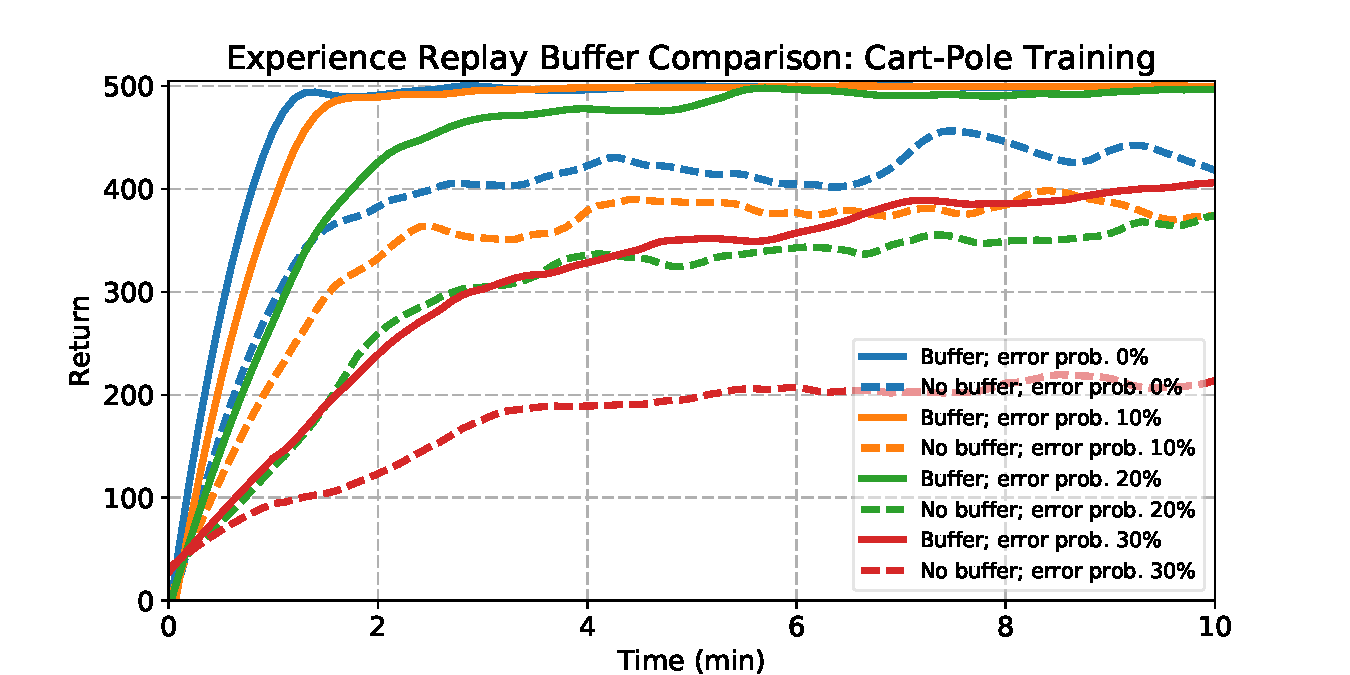
\includegraphics[width=0.66\linewidth]{imagenes/cap3/buffer_cart_pole.pdf}
    \vspace{-0.2cm}
    \caption[Comparison between using or not experience replay buffer for different values of $P_\mathit{err}$ in the Cart-Pole problem.]{Comparison between using or not experience replay buffer for different values of $P_\mathit{err}$ in the Cart-Pole problem. Buffer: $K = 200$; $b = 10$; $N = 50$. $P_{h}$: $\alpha = 0.6$; $\tau = 0.0003$; $\emph{e}=1$. Simulated teacher network learning rate: $0.0003$.}
    \label{fig:buffer_cart_pole}
    \vspace{-0.2cm}
\end{figure}

\begin{figure}[H]
    \centering
    \vspace{-0.2cm}
    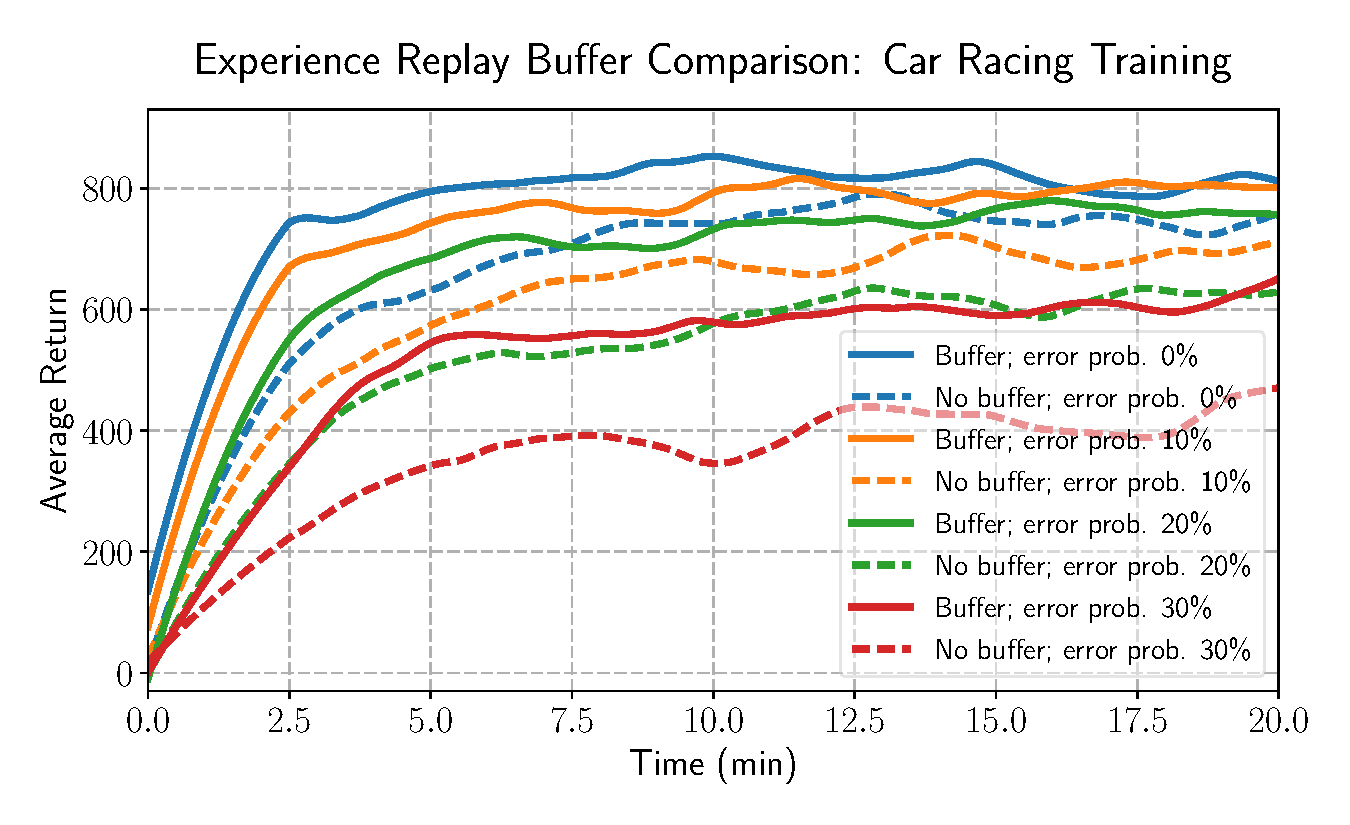
\includegraphics[width=0.66\linewidth]{imagenes/cap3/bufferCarRacing.pdf}
    \vspace{-0.2cm}
    \caption[Comparison between using or not experience replay buffer for different values of $P_\mathit{err}$ in the Car Racing problem.]{Comparison between using or not experience replay buffer for different values of $P_\mathit{err}$ in the Car Racing problem. Buffer: $K = 1000$; $b = 10$; $N = 100$. $P_{h}$: $\alpha = 0.6$; $\tau = 0.000015$; $\emph{e}=(1, 1, 1)$. Simulated teacher network learning rate: $0.0003$.}
    \label{fig:buffer_car_racing}
    \vspace{-0.2cm}
\end{figure}

In \figurename~{\ref{fig:buffer_cart_pole}} and \figurename~{\ref{fig:buffer_car_racing}} the learning curves show a large difference between the processes of learning that use experience replay buffer with respect to the cases without the buffer. In the case without the buffer, which is more similar to the original COACH, it is possible to see that the learning agent is not benefiting from the advised corrections as much as it can do when the pieces of advice are kept in the memory. For instance, we can see that $\text{D-COACH OFF}$ learns more from corrections with $20 \%$ of mistakes when using the buffer than in the case of perfect corrections, but without any buffering. This means the buffer is necessary for increasing the use of the available information, even when this information could be corrupted and not clean.

\subsection{Comparison of DRL and D-COACH OFF using real human teachers}

These experiments are intended to compare the learning process of D-COACH OFF (simulated teacher and human teacher) with the DRL algorithm DDPG. Taking into account that the Cart-Pole problem has a low dimensional state space, the original COACH, based on basis functions, is also included in the comparison. In this case, $P_\mathit{err}=0\%$ was used for the simulated teachers. The results of this problem are shown in \figurename~{\ref{fig:cartpole_results}}, wherein it is possible to see that COACH-like methods outperform the DDPG agent with a large difference. When using the simulated teacher, D-COACH OFF learns faster than the original COACH. The performance of D-COACH OFF with human teachers decreases with respect to the simulated teacher. This is because human teachers are not perfect and make mistakes, but they are being compared with a simulated teacher with $P_\mathit{err}=0\%$, which means that it makes no mistakes. Also, because the simulated teacher model is quite simple to represent the complexity of the human behavior, then, although it is not very realistic, it is still useful for comparisons of interactive learning strategies under similar conditions.

\begin{figure}[h]
    \centering
    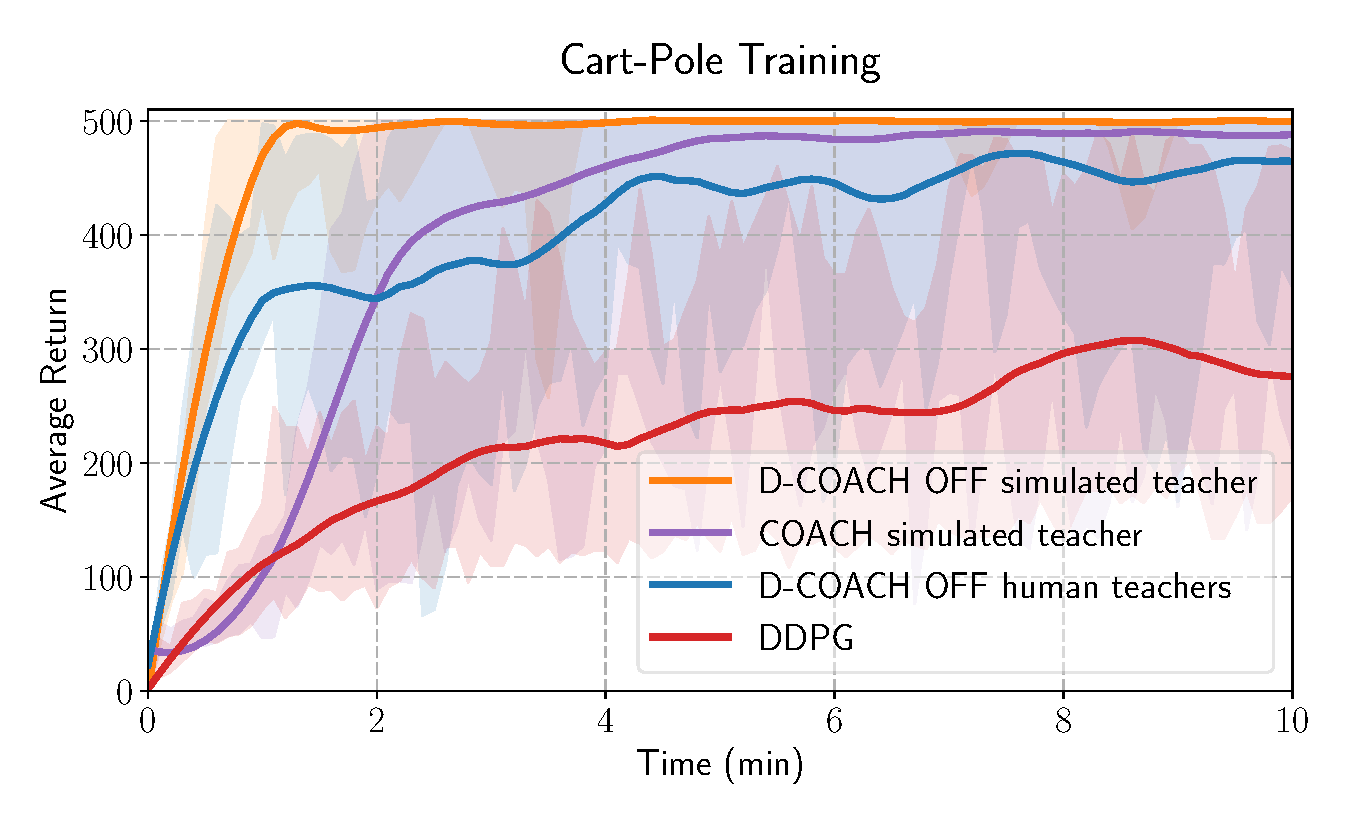
\includegraphics[width=0.7\linewidth]{imagenes/cap3/offline_cart_pole_humans.pdf}
    \caption[Cart-Pole training.]{Cart-Pole training. Buffer: $K = 200$; $b = 10$; $N = 50$. $P_{h}$: $\alpha = 0.6$; $\tau = 0.0003$; $\emph{e}=1$. Human teacher network learning rate: $0.003$; Simulated teacher network learning rate: $0.0003$.}
    \label{fig:cartpole_results}
\end{figure}

In \figurename~{\ref{fig:racing_car_results1}} the learning curves of the Car Racing problem are presented. Again, D-COACH OFF results in a fast convergence. Unlike reported results of DRL algorithms for this problem (see Table \ref{CarRacing_table}), in the very early minutes D-COACH OFF reaches high performance policies that have not been obtained by most of the DRL approaches, to the best of our knowledge. If we compare a policy trained with D-COACH OFF for approximately 75 minutes by an experienced teacher against several state-of-the-art DRL approaches, it can be seen that it outperforms most of them. The problem is considered to be solved if the agent gets an average score of 900 or more over 100 random tracks. However, we observed that this value can substantially vary between different evaluations, so in Table \ref{CarRacing_table}, the obtained range of values over 20 evaluations is presented for D-COACH OFF.

\begin{figure}[h]
    \centering
    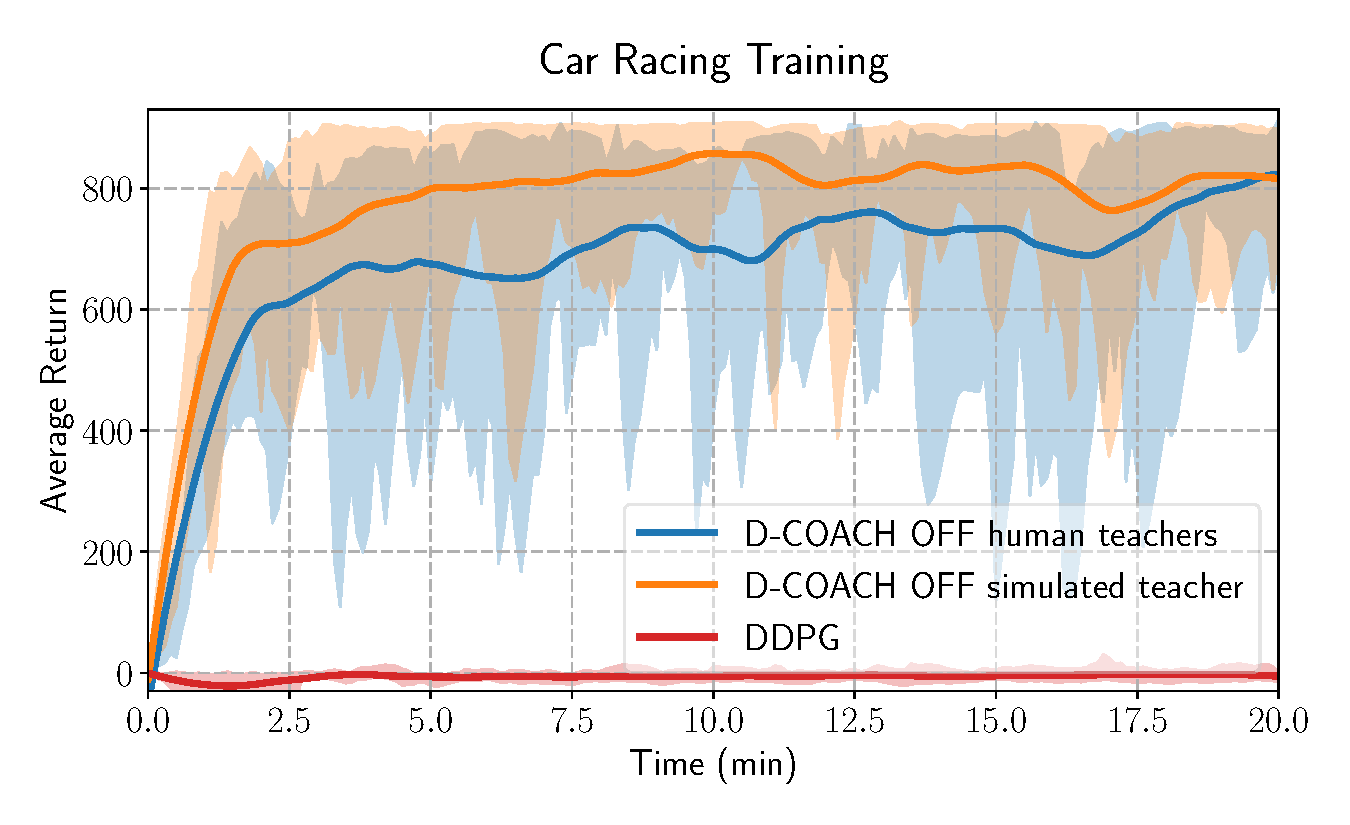
\includegraphics[width=0.7\linewidth]{imagenes/cap3/offline_car_racing_humans.pdf}
    \caption[Car Racing training.]{Car Racing training. Buffer: $K = 1000$; $b = 10$; $N = 100$. $P_{h}$: $\alpha = 0.6$; $\tau = 0.000015$; $\emph{e}=(1, 1, 1)$. Human teacher network learning rate: $0.001$; Simulated teacher network learning rate: $0.0003$.}
    \label{fig:racing_car_results1}
\end{figure}

\begin{table}[h]
\centering
\caption[Car Racing state-of-the-art learning algorithms comparison.]{Car Racing state-of-the-art learning algorithms comparison. DRL results taken from (Ha \& Schmidhuber, 2018) \cite{Ha2018}.}
\label{CarRacing_table}
\begin{tabular}{lc}
\multicolumn{1}{c}{\textbf{Method}}      & \multicolumn{1}{l}{\textbf{Average Score over 100 Random Tracks}} \\ \hline\hline
DQN                                      & 343 $\pm$ 18                                                      \\ \hline
A3C (continuous)                         & 591 $\pm$ 45                                                      \\ \hline
A3C (discrete)                           & 652 $\pm$ 10                                                      \\ \hline
ceobillionaire’s algorithm (unpublished) & 838 $\pm$ 11                                                      \\ \hline
Full World Model                         & 906 $\pm$ 21                                                      \\ \hline
\textbf{D-COACH OFF (experienced teacher)}                         & \textbf{895 - 909 $\pm$ 18 - 80} \\
& \textbf{Average over 20 evaluations: 903 $\pm$ 46}
\\ \hline
\end{tabular}
\end{table}

\newpage

\subsection{Validation in a real system}
In the third problem that we called Duckie Racing, an agent has to learn to drive a Duckiebot (from the project  Duckietown \cite{Paull2017} with modifications from the Chile Duckietown Team\footnote{\url{https://github.com/Duckietown-Chile/}}) autonomously through a track based on raw visual information of an onboard camera. The actions in this problem are the forward speed and the steering angle of the Duckiebot. Two tasks are set for this environment: (i) driving the Duckiebot freely through the track, with permission to drive in both lanes, and (ii) driving the Duckiebot only in the right lane, which demands more accuracy in driving. In this problem, an episode stops if the robot leaves the track/right lane, or after 30 seconds. The performance index in this task is the percentage of the total track length traveled during the episode. Hence the faster and more accurate the Duckiebot drives, the more distance it will travel.

This problem is not used for comparisons of the methods, but only as a validation of D-COACH OFF using experience replay, which showed to be the best alternative in the previous problems. \figurename~\ref{fig:racing_duckie_results} shows the learning curve for each of the tasks explored in this environment with a real robot and a real human teacher. The curves and the following video \url{https://youtu.be/vcEtuRrRIe4} show that the system quickly learns to drive properly through the road based only on the human corrections. As expected, the policy is faster when the robot has the freedom to drive over both lanes. Learning this task with RL would definitely take more training time, and might need an external perception system to compute the reward function, whereas with D-COACH this performance index does not have any influence on the learning process, rather it is used for descriptive and comparative purposes.

\begin{figure}[h]
    \centering
    \begin{minipage}{.5\textwidth}
    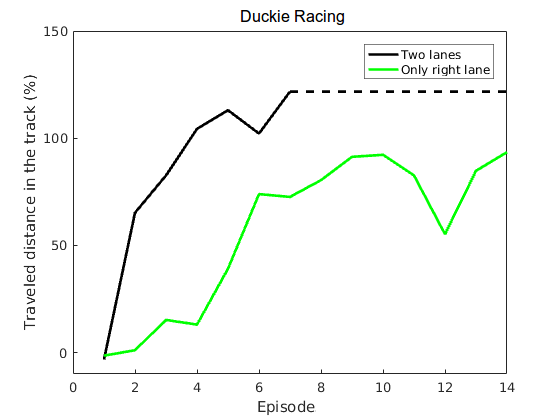
\includegraphics[width=1.0\linewidth]{imagenes/cap3/racing_duckie_results.png}
    \vspace{-0.2cm}
    \caption[Duckie Racing training.]{Duckie Racing training. A traveled distance of 100\% indicates that the car finished one lap. The experiment lasted less than 7 minutes. $K = 1000$; $k=20$; $b = 10$; $N = 8$. $\emph{e}=(1, 1)$;. Human teacher network learning rate: $0.003$.}
    \label{fig:racing_duckie_results}
    \end{minipage}%
    \begin{minipage}{.5\textwidth}
    \centering
    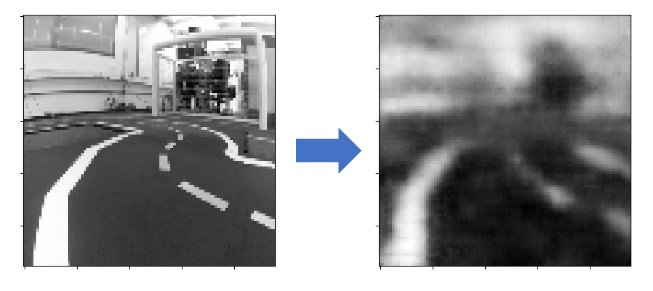
\includegraphics[width=1.0\linewidth]{imagenes/cap3/AE_duckie2.png}
    \caption[Duckie Racing autoencoder input vs output.]{Duckie Racing autoencoder input (left) vs output (right).}
    \label{fig:AE_duckie}
    \end{minipage}
\end{figure}

\vspace{1cm}

\section{Discussion}
This chapter presented D-COACH (D-COACH OFF specifically), an algorithm for training policies modeled with DNNs interactively with corrective advice. The method was validated in a problem of low-dimensionality, along with problems of high-dimensional state spaces like raw pixel observations, with a simulated and a real robot environment, and also using both simulated and real human teachers. 

The use of the experience replay buffer (which has been well tested for DRL) was validated for this different kind of learning approach, since this is a feature not included in the original COACH. The comparisons showed that the use of memory resulted in an important boost in the learning speed of the agents, which were able to converge with less feedback, and to perform better even in cases with a significant amount of erroneous signals.  

The results of the experiments verify that teachers advising corrections can train policies in fewer time steps than a DRL method like DDPG. So it was possible to train real robot tasks based on human corrections during the task execution, in an environment with a raw pixel level state space. 

The comparison of D-COACH with respect to DDPG, shows how this interactive method makes it more feasible to learn policies represented with DNNs, within the constraints of physical systems. DDPG needs to accumulate millions of time steps of experience in order to obtain good performances as shown in \cite{Lillicrap2015}. However, this is not always possible with real systems.